% !TeX root = Protokoll.tex

Für die Untersuchung der Materialien der drei tomographierten Würfel wurden mit Hilfe des Szintillationsdetektors
und des Multichannel Analyser die Spektren der Gamma-Strahlung nach der Durchdringung des jeweiligen Würfels
aufgenommen. Eines dieser Spektren ist in \cref{fig:spektrum_block_1_messung_5_0_350_histogram_intervall} dargestellt.
In dieser Abbildung ist der Bereich des Gesamtenergie-Peaks farblich hervorgehoben. Über diesen Bereich 
der Kanäle von 250 bis 310 wurden die gemessenen Hits jeder Messreihe integriert. Da die Integration immer über 
diesen Bereich durchgeführt wird sind die gemessenen Anzahlen in jeder Messreihe proportional zur Intensität der 
gemessenen Strahlung. Da für die Auswertung nur die Verhältnisse der Intensitäten benötigt werden, können diese
durch die Verhältnisse der gemessenen Anzahlen ersetzt werden.
Diese Werte befinden sich 
für jede verwendete Projektion in den Tabellen \ref{tab:Messung_I1},\ref{tab:Messung_I2} und \ref{tab:Messung_I3}. 
Die Werte in \cref{tab:Messung_I0} wurden bei der Messung des holen Aluminiumwürfels aufgenommen, um 
einen Referenzwert $I_{0}$ bestimmen zu können.
 
\begin{figure}[!h]
 \centering
 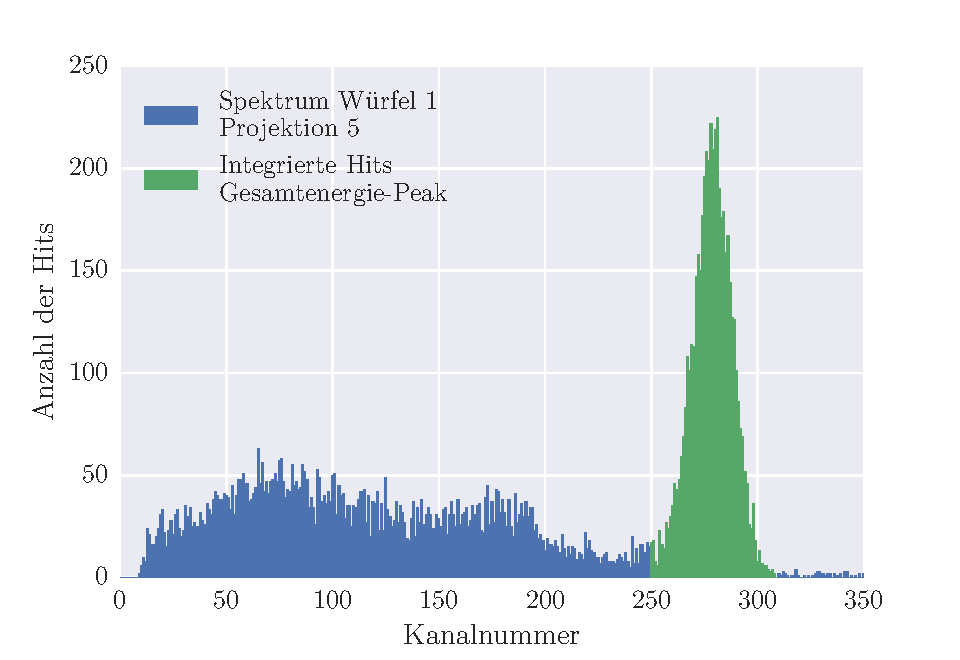
\includegraphics[scale=0.90]{../Grafiken/Spektrum_Block_1_Messung_5_0_350_histogram_intervall.pdf}
 \caption{Beispielhafte Darstellung eines mit dem MCA aufgenommenen 
 	Spektrums. Dabei ist hier nur ein Ausschnitt der 1024 Kanäle gezeigt, da in dem nicht gezeigten Bereich  
 	sehr wenige und nicht relevante Hits aufgenommen wurden. Im speziellen handelt es sich um das Spektrum welche bei der 5. 
 	Projektion der Messung mit Würfel 1 aufgenommen wurde. In grün hervorgehoben ist der Bereich des 
 	Gesamtenergie-Peaks, über den die Anzahl der Hits integriert wurde, um die Materialien der untersuchten 
 	Würfel zu bestimmen.  
 	\label{fig:spektrum_block_1_messung_5_0_350_histogram_intervall}}
 \end{figure}  

\begin{table}[!h]
	\centering
	\begin{tabular}{cccccc}
		\toprule
		Projektion & Messzeit & Int. Anzahl Hits & Projektion & Messzeit & Int. Anzahl Hits\\
		$j$ & $t$/\si{\second} & $I_j$ & $j$ & $t$/\si{\second} & $I_j$\\
\midrule
		\num{1} & \num{119.660} & \num{29255(171)} & \num{7} & \num{119.640} & \num{29019(170)}\\
		\num{2} & \num{119.640} & \num{29148(171)} & \num{8} & \num{119.620} & \num{29340(171)}\\
		\num{3} & \num{119.660} & \num{29050(170)} & \num{9} & \num{119.680} & \num{29334(171)}\\
		\num{4} & \num{119.600} & \num{29966(173)} & \num{10} & \num{119.640} & \num{29541(172)}\\
		\num{5} & \num{119.680} & \num{29639(172)} & \num{11} & \num{119.580} & \num{29899(173)}\\
		\num{6} & \num{119.640} & \num{28691(169)} & \num{12} & \num{119.660} & \num{29615(172)}\\
		\bottomrule
	\end{tabular}
	\caption{Integrierte Anzahl der Hits und Messzeit  für die 
                      verschiedenen Projektionen $P_{j}$ für die Untersuchung eines mit Luft 
                      gefüllten Aluminiumwürfels. \label{tab:Messung_I0}}
\end{table}


  
Durch Mittlung der Messwerte der Referenzmessung ergibt sich eine Referenzanzahl von $I_{0} = \num{29374(171)}$ 
und eine gemittelte Messzeit von $\overline{t_{0}} = \SI{119.642}{\second}$. Diese Messzeit wird im weiteren dazu
verwendet, die Referenzmessung jeweils auf die Messzeit der drei folgenden Messreihen zu normieren.
Diese Normierung auf die Projektion $j$ einer Messreihe erfolgt nach
\begin{empheq}{equation}
	I_{0,j} = I_{0} \cdot \frac{t_{j}}{\overline{t_{0}}}.
\end{empheq}

Die logarithmierten Verhältnisse $N_{j}$ dieser normierten Referenzanzahl und der jeweiligen Anzahlen aus den durchgeführten Messreihen ergeben sich nach 
\begin{empheq}{equation}
N_{j} = \ln(\frac{I_{0,j}}{I_j})
\end{empheq}
und sind in \cref{tab:Messung_Verhaeltnis} angegeben. Die mit diesen Werten angegebenen Fehler berechnen sich unter
Verwendung der Gaußschen-Fehlerfortpflanzung \cref{eq:Fehlerforpflanzung} aus der Gleichung

\begin{empheq}{equation}
\sigma_{N_{j}} = \sqrt{\del{\dfrac{\sigma_{I_{0,j}}}{I_{0,j}}}^2 + \del{\dfrac{\sigma_{I_j}}{I_j}}^2}.
\end{empheq}

Über die in \cref{eq:KleinsteQuadrate} dargestellte \enquote{Methode der Kleinsten Quadrate} ergeben sich die in 
\cref{tab:Absorbtionskoeffizienten} eingetragenen Absorptionskoeffizienten. Die angegebene Fehler wurden 
entsprechend nach \cref{eq:KleinsteQuadrateFehler} bestimmt.

\FloatBarrier
\begin{table}[!h]
	\centering
	\begin{tabular}{cccccc}
		\toprule
		Projektion & Messzeit & Int. Anzahl Hits & Projektion & Messzeit & Int. Anzahl Hits\\
		$j$ & $t$/\si{\second} & $I_j$ & $j$ & $t$/\si{\second} & $I_j$\\
\midrule
		\num{1} & \num{119.800} & \num{4503(67)} & \num{7} & \num{119.760} & \num{6046(78)}\\
		\num{2} & \num{119.680} & \num{2978(55)} & \num{8} & \num{119.820} & \num{3073(55)}\\
		\num{3} & \num{119.740} & \num{6396(80)} & \num{9} & \num{119.740} & \num{4990(71)}\\
		\num{4} & \num{119.800} & \num{5013(71)} & \num{10} & \num{119.720} & \num{4920(70)}\\
		\num{5} & \num{119.660} & \num{4969(71)} & \num{11} & \num{119.680} & \num{4918(70)}\\
		\num{6} & \num{119.760} & \num{5458(74)} & \num{12} & \num{119.680} & \num{5422(74)}\\
		\bottomrule
	\end{tabular}
	\caption{Integrieter Anzahl der Hits und Messzeit für die verschiedenen Projektionen $j$ für die
Untersuchung von Würfel 1.  \label{tab:Messung_I1}}
\end{table}

\FloatBarrier
\begin{table}[!h]
	\centering
	\begin{tabular}{cccccc}
		\toprule
		Projektion & Messzeit & Int. Anzahl Hits & Projektion & Messzeit & Int. Anzahl Hits\\
		$j$ & $t$/\si{\second} & $I_j$ & $j$ & $t$/\si{\second} & $I_j$\\
\midrule
		\num{1} & \num{328.220} & \num{2994(55)} & \num{7} & \num{328.040} & \num{3220(57)}\\
		\num{2} & \num{328.120} & \num{1296(36)} & \num{8} & \num{327.820} & \num{1323(36)}\\
		\num{3} & \num{328.760} & \num{5373(73)} & \num{9} & \num{328.680} & \num{4363(66)}\\
		\num{4} & \num{328.700} & \num{3239(57)} & \num{10} & \num{328.740} & \num{3224(57)}\\
		\num{5} & \num{328.620} & \num{2978(55)} & \num{11} & \num{328.480} & \num{3099(56)}\\
		\num{6} & \num{328.520} & \num{3603(60)} & \num{12} & \num{328.820} & \num{4188(65)}\\
		\bottomrule
	\end{tabular}
	\caption{Integriete Anzahl der Hits und Messzeit für die verschiedenen Projektionen $P_{j}$ für die 
Untersuchung von Würfel 2.  \label{tab:Messung_I2}}
\end{table}

\FloatBarrier
\begin{table}[!h]
	\centering
	\begin{tabular}{cccccc}
		\toprule
		Projektion & Messzeit & Int. Anzahl Hits & Projektion & Messzeit & Int. Anzahl Hits\\
		$j$ & $t$/\si{\second} & $I_j$ & $j$ & $t$/\si{\second} & $I_j$\\
\midrule
		\num{1} & \num{179.460} & \num{3472(59)} & \num{7} & \num{179.620} & \num{9887(99)}\\
		\num{2} & \num{177.060} & \num{2618(51)} & \num{8} & \num{179.500} & \num{2523(50)}\\
		\num{3} & \num{179.620} & \num{9747(99)} & \num{9} & \num{179.400} & \num{3633(60)}\\
		\num{4} & \num{179.540} & \num{4183(65)} & \num{10} & \num{179.440} & \num{4267(65)}\\
		\num{5} & \num{179.220} & \num{4173(65)} & \num{11} & \num{179.620} & \num{4117(64)}\\
		\num{6} & \num{179.660} & \num{4688(69)} & \num{12} & \num{179.460} & \num{4354(66)}\\
		\bottomrule
	\end{tabular}
	\caption{Integrieter Anzahl der Hits und Messzeit für die verschiedenen Projektionen $j$ für die
Untersuchung von Würfel 3.  \label{tab:Messung_I3}}
\end{table}

\FloatBarrier
\begin{table}[!h]
	\centering
	\begin{adjustbox}{width=\textwidth}
\begin{tabular}{cccc}
	\toprule
	Projektion & log. Verhältnis Würfel 1 & log. Verhältnis Würfel 2 & log. Verhältnis Würfel 3\\
	$j$ & $N_{1,j}$ & $N_{2,j}$ & $N_{3,j}$\\
	\midrule
	\num{1} & \num{1.88(2)} & \num{3.29(2)} & \num{2.54(2)}\\
	\num{2} & \num{2.29(2)} & \num{4.13(3)} & \num{2.81(2)}\\
	\num{3} & \num{1.53(1)} & \num{2.71(1)} & \num{1.51(1)}\\
	\num{4} & \num{1.77(2)} & \num{3.22(2)} & \num{2.36(2)}\\
	\num{5} & \num{1.78(2)} & \num{3.30(2)} & \num{2.36(2)}\\
	\num{6} & \num{1.68(1)} & \num{3.11(2)} & \num{2.24(2)}\\
	\num{7} & \num{1.58(1)} & \num{3.22(2)} & \num{1.50(1)}\\
	\num{8} & \num{2.26(2)} & \num{4.11(3)} & \num{2.86(2)}\\
	\num{9} & \num{1.77(2)} & \num{2.92(2)} & \num{2.50(2)}\\
	\num{10} & \num{1.79(2)} & \num{3.22(2)} & \num{2.33(2)}\\
	\num{11} & \num{1.79(2)} & \num{3.26(2)} & \num{2.37(2)}\\
	\num{12} & \num{1.69(1)} & \num{2.96(2)} & \num{2.31(2)}\\
	\bottomrule
\end{tabular}
	\end{adjustbox}
	\caption{Logarithmiertes Verhältnis der gemittelten Maximalintensität $I_0$ und den gemessenen  
integrierten Anzahlen der Hits $I_j$ für die Messungen mit den drei Würfeln. Die Maximalintensität $I_0$ wurde dabei 
jeweils auf die Messzeiten der jeweiligen Messung normiert. \label{tab:Messung_Verhaeltnis}}
\end{table}

\FloatBarrier
\begin{table}[!h]
	\centering
\begin{adjustbox}{width=\textwidth}
	\begin{tabular}{cccc}
		\toprule
		Elementarwürfel & Abs. Koeffizient Würfel 1 & Abs. Koeffizient Würfel 2 & Abs. Koeffizient Würfel 3\\
		$i$ & $\mu_{1,i}$ & $\mu_{2,i}$ & $\mu_{3,i}$\\
\midrule
		\num{1} & \num{0.516(9)} & \num{0.95(1)} & \num{0.78(1)}\\
		\num{2} & \num{0.521(7)} & \num{0.880(8)} & \num{0.679(7)}\\
		\num{3} & \num{0.393(9)} & \num{0.76(1)} & \num{0.42(1)}\\
		\num{4} & \num{0.477(7)} & \num{0.961(8)} & \num{0.352(6)}\\
		\num{5} & \num{0.499(8)} & \num{0.87(1)} & \num{0.648(8)}\\
		\num{6} & \num{0.649(7)} & \num{1.056(8)} & \num{1.030(8)}\\
		\num{7} & \num{0.533(9)} & \num{0.84(1)} & \num{0.80(1)}\\
		\num{8} & \num{0.569(7)} & \num{1.147(8)} & \num{0.681(7)}\\
		\num{9} & \num{0.394(9)} & \num{0.65(1)} & \num{0.47(1)}\\
		\bottomrule
	\end{tabular}
\end{adjustbox}
	\caption{Unter Verwendug der Methode der kleinsten Quadrate bestimmte Absorbtionskoeffizeinten 
und deren Fehler der jeweils neun Elementarwürfel in den vermessenen drei Würfeln. \label{tab:Absorbtionskoeffizienten}}
\end{table}

\FloatBarrier
Da die ersten beiden Messreihen mit Würfeln durchgeführt wurden, die nur aus einem Material bestehen,
ergeben sich die Absorptionskoeffizienten dieser Materialien durch Mittlung der neun bestimmten Absorptionskoeffizienten zu 
\begin{empheq}{align}
\overline{\mu}_{W1} &= \SI{0.505(3)}{\per\centi\metre} \\
\overline{\mu}_{W2} &= \SI{0.902(3)}{\per\centi\metre} .
\end{empheq}


\begin{table}[!h]
	\centering
	\begin{tabular}{lccc}
		\toprule
		Material & Dichte & Skalierter Abs. Koeffizient\cite{XCOM} & Abs. Koeffizient\\
		$$ & $\rho$/\si{\gram\per\centi\metre\cubed} & $\frac{\mu}{\rho}$/\si{\centi\metre\squared\per\gram} & $\mu$/\si{\per\centi\metre}\\
\midrule
		Aluminium & \num{2.7}\,\cite{ChemMaster} & \num{0.075} & \num{0.202}\\
		Blei & \num{11.3}\,\cite{ChemMaster} & \num{0.110} & \num{1.245}\\
		Delrin & \num{1.4}\,\cite{MDC} & \num{0.082} & \num{0.115}\\
		Eisen & \num{7.9}\,\cite{ChemMaster} & \num{0.073} & \num{0.580}\\
		Messing & \num{8.5}\,\cite{ChemMaster} & \num{0.073} & \num{0.619}\\
		\bottomrule
	\end{tabular}
	\caption{Absorbtionskoeffizenten und Dichten der Materialien, aus denen die untersuchten Würfel
aufgebaut sein können. \label{tab:Materialien}}
\end{table}


Im Vergleich der Messergebnisse mit den Literaturwerten zeigt sich, dass keines der Materialien 
eindeutig zugeordnet werden kann. Jedoch ist durch die Größenordnung der bestimmten Absorptionskoeffizienten
anzunehmen, dass es sich bei Würfel 1 um das Material Messing und bei Würfel 2 um Blei handelt.
Für Würfel 1 ergibt sich damit eine relative Abweichung 
%$\Delta_{\mathrm{rel}}\mu_{1,\mathrm{Fe}} \approx \SI{13}{\percent}$ bzw.
$\Delta_{\mathrm{rel}}\mu_{1,\mathrm{CuZn}} \approx \SI{18}{\percent}$. 
Die relative Abweichung des Ergebnisses für den zweiten Würfel
beträgt in etwa $\Delta_{\mathrm{rel}}\mu_{1,\mathrm{Pb}} \approx \SI{28}{\percent}$.
Unterzieht man die neun Absorptionskoeffizienten der Elementarwürfel in Würfel 3 dem Vergleich mit den 
Werten für Würfel 1 und Würfel 2,
so ergibt sich die Zuordnung der Materialien zu den Elementarwürfeln in \cref{tab:Materialien_Block3}.
Der Vergleich wird mit den im Versuch bestimmten Absorbtionskoeffizienten durchgeführt,
da für die Messung des dritten Würfels Abweichungen in der gleichen Größenordnung zu erwarten sind. 

\begin{table}[!h]
	\centering
\begin{adjustbox}{width=\textwidth}
	\begin{tabular}{clcclc}
		\toprule
		Elementarwürfel & Material & rel. Abweichung & Elementarwürfel & Material & rel. Abweichung\\
		$i$ & & $\Delta_{rel}\mu/\%$ & $i$ & &$\Delta_{rel}\mu /\%$\\
\midrule
		\num{1} & Messing & \num{26}   & \num{6}& Blei& \num{17}\\
		\num{2} & Messing & \num{10}& \num{7}& Messing / Blei & \num{29}/\num{36}\\
		\num{3} & Eisen / Messing  &\num{29}/\num{33} &\num{8}& Messing & \num{10}\\
		\num{4} & Eisen/Messing & \num{39}/\num{43}  & \num{9}& Eisen& \num{20}\\
		\num{5} & Messing & \num{5} &  &   &  \\
		
		\bottomrule
	\end{tabular}
\end{adjustbox}
	\caption{Zuordnung der möglichen Materialien zu den Einheitswürfeln des Würfels 3
		durch Vergleich der Absorptionskoeffizienten mit den Literaturwerten. Liegt das Messergebnis 
		zwischen zwei Literaturwerten so wurden beide möglichen Materialien angegeben, wobei das erste den
		geringeren Unterschied zum Messwert aufweist. \label{tab:Materialien_Block3}}
\end{table}
